% PARTIE 1 - PRESENTATION %%%%%%%%%%%
% CHAPITRE 1 %%%%%%%%%%%%%%%%%%%%%%%%
%%%%%%%%%%%%%%%%%%%%%%%%%%%%%%%%%%%%%
Ce chapitre premier, introductif, présente le contexte historique du projet de recherche: son objet d'étude, ses acteurs, ses corpus de recherche et ses objectifs. Le cadre historique dans lequel le projet s'inscrit est également exposé sous le prisme de la gestion de projet. 

%%%%%%%%%%%%%%%%%%%%%%%%%%%%%%%%%%%%%
% SECTION %%%%%%%%%%%%%%%%%%%%%%%%%%%
\section{Définition historique du projet Richelieu}
\enquote{Le quartier Richelieu existe-t-il?}\footcite{DUVETTEquartier2024} Administrativement, le quartier Richelieu n'exis\-te pas. Il n'est pas et n'a jamais été une subdivision du 2\ieme~  arrondissement de la ville de Paris. Historiquement, le quartier Richelieu, tel qu'il a été défini par les historiennes du projet, ne correspond pas aux censives d'Ancien Régime, ni aux sections révolutionnaires parisiennes\footcite{VOVELLEsections1988} et encore moins à la restructuration des quartiers précédents le Second Empire. Donc il ne correspond ni aux normes administratives contemporaines ni aux quadrillages urbains anciens. 

\begin{figure}
    \centering
    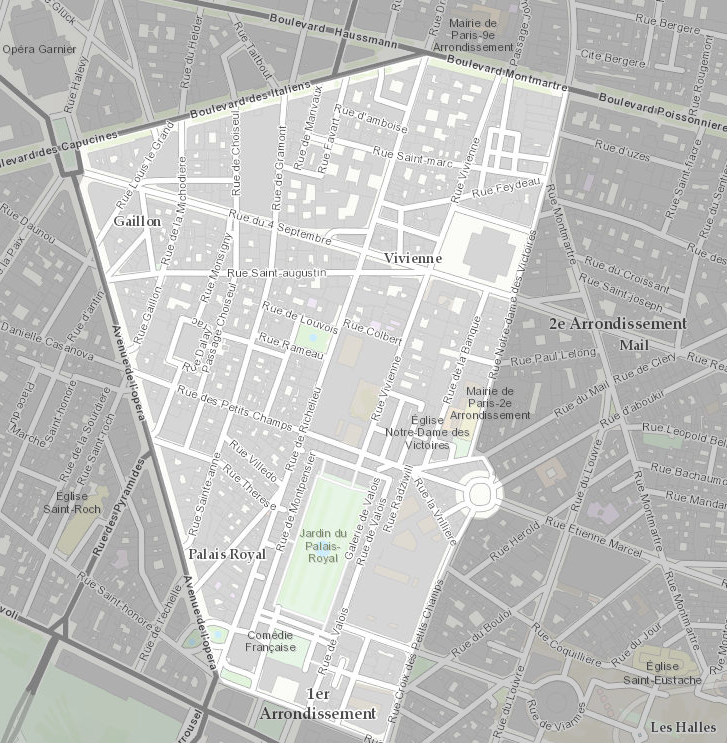
\includegraphics[width=0.5\linewidth]{images/Emprise_quartier_Richelieu.png}
    \caption{Emprise du quartier Richelieu, \mhd.}
    \label{fig:emprise_quartier}
\end{figure}

Au contraire, \enquote{Richelieu}, à comprendre comme un nom d'usage, se situe dans les quartiers Vivienne et Gaillon pour le 2\ieme~  arrondissement et dans le quartier du Palais Royal pour le 1er arrondissement. Ses axes principaux sont les rues des Petits-Champs, Richelieu, Vivienne. Il est ainsi délimité par des ensembles architecturaux tels que le Palais-Royal, l'Opéra Garnier, les grands Boulevards, la place de la Bourse et la place des Victoires (voir la figure \ref{fig:emprise_quartier})\footcite{INHACarnet2023}.

\begin{figure}
    \centering
    \includegraphics[width=0.5\linewidth]{images/BnF_quartier_Richelieu.jpeg}
    \caption{Affiche \textit{Paris, quartier Richelieu. Principales maisons de l'industrie, principales maisons du commerce} ... [placard d'annonces publicitaires pour différents commerces], 1862, Bibliothèque nationale de France, département Estampes et photographie, ENT DP-267-ROUL.}
    \label{fig:richelieu_pub}
\end{figure}


Pourquoi alors utiliser une dénomination qui \textit{a priori} n'existe pas ? En premier lieu, quelques usages ont été retrouvés dans les sources historiques: le nom est utilisé sur certaines affiches publicitaires des années 1860 (voir la figure \ref{fig:richelieu_pub}), sans doute en référence à la rue de Richelieu qui traverse le quartier. Mais quelques occurrences ne suffisent pas à donner un titre à tout un quartier. 

Surtout, ce titre renvoie aux institutions porteuses du projet Richelieu loties dans le \enquote{Quadrilatère Richelieu} ou \enquote{site Richelieu}\footcite{BNFquadrilatere2024}. Berceau historique de la \acrlong{bnf}, le site est un millefeuille architectural situé au cœur de Paris. Il est bordé à l'ouest par la rue Richelieu, au nord par la petite rue Colbert, à l'est par la rue Vivienne et au sud par la rue des Petits-Champs. Le site Richelieu a évolué au fil des siècles en passant du XVII\ieme~ siècle au XX\ieme~ siècle d'une résidence privée du cardinal Mazarin à un édifice devenu public abritant d'abord la bibliothèque royale, puis la \acrshort{bnf}\footcite{BNFLhistoire2023}. En réponse à l'évolution des besoins, la rénovation du site Richelieu, menée sur 12 ans, a entièrement réorganisé l'espace pour le consacrer à l'histoire des arts et du patrimoine. En plus des départements spécialisés de la \acrlong{bnf}, le site accueille désormais la bibliothèque de l'\acrlong{inha} et celle de l'\acrlong{enc}. Enfin, le titre du projet est le reflet d'une nouvelle clé de lecture du quartier proposée par les chercheurs, qui est au cœur de l'objet d'étude du projet de recherche. 

\section{L'objet d'étude : un enjeu historiographique}

Tout d'abord, la notion de \enquote{quartier} est historiquement remise en question. Que signifie \enquote{faire quartier}? Comme pour de nombreuses frontières nationales, les délimitations administratives des quartiers ne représentent pas les relations du voisinage, car les frontières d'un quartier \enquote{fluctuent d'un individu à l'autre}.\footnote{\enquote{Le quartier}, \textit{Le peuple de Paris au XIX\ieme~  siècle}, Miriam SIMON (dir.), Paris, Paris Musées, 2011, p.182.}\footcite{JAKOBOWICZpeuple2011} 
Quels sont alors les éléments historiques qui confèrent au quartier Richelieu son identité en tant que quartier ?  Contrairement à d'autres quartiers parisiens ou limitrophes, cet espace géographique est souvent négligé dans l'historiographie, bien qu'il se distingue par son histoire urbaine, ses activités économiques, culturelles\footcite{GRESILLONVille2008} et sociales\footcite{DIMEOgeographie2008, INHAJournee2023, INHAJournee2023a}, ainsi que par son architecture et ses usages. Sur une période de deux siècles, de 1750 à 1950, ce quartier, situé en plein cœur de Paris, a été au centre des évolutions modernes. Les institutions présentes et les aménagements urbains y ont joué un rôle majeur, notamment le \enquote{Quadrilatère Richelieu}, la Banque de France, le Palais Brongniart, le Palais Royal, le Conseil d'État, ainsi que d'autres organismes comme l'Agence France Presse. Les îlots du quartier se transforment petit à petit et non dans leur globalité, à l'instar des grands travaux de rénovation motivés par le baron Haussmann. Bien que les transformations urbaines du quartier soient ponctuelles et étalées dans le temps et l'espace\footcite{CARBONNIERderoulement2015}, il conserve une identité, une valeur culturelle et matérielle ancrée dans ses activités distinctes.

Le passage suivant, tiré d'un guide de Paris\footnote{Charles JOLIET \enquote{Les petites caves, les petites cuisines}, dans, \textit{Paris-Guide}, par les principaux écrivains et artistes de la France ; introduction par Victor Hugo, Paris, librairie internationale, 1867, p. 1558-1559. in \footcite{DUVETTEquartier2024}} de la seconde moitié du XIX\ieme~  siècle, permet d'en prendre le pouls : 

\begin{displayquote}\enquote{Cette rue est la rue Vivienne, la plus brillante et la plus animée. C'est Paris avec sa fièvre et ses mirages. Le centre topographique est la place du Châtelet, mais le vrai centre est ici. Chaque seconde, marquée par l'horloge de la Bourse, compte les pulsations du cœur de l'Europe. À cette extrémité, le Palais-Royal [...], à l'autre, le boulevard. De ce centre, en décrivant une circonférence restreinte, on englobe dix théâtres [...]. Ce monument bâti en briques et en pierres de taille déployant sa double façade, c'est la Bibliothèque qui renferme dans ses catalogues l'héritage de toutes les littératures [...]. Chaque boutique qui sollicite ton regard est une exposition spéciale et choisie. Voici une machine à vapeur, des objets d'art, l'antiquité et la mode ; là une boutique de libraire, le musée de la gastronomie, un magasin de fleurs, des tableaux, des gravures, des bronzes, les photographies des célébrités des lettres, des sciences, des arts, de la chaire, du barreau, de la politique, de la cour, de la ville et du théâtre ; dans ce kiosque, cent journaux ; devant toi la poste et le télégraphe : ici, des hôtels, des cercles, des cafés, des passages. En deux heures avec l'or que nous n'avons pas, on peut y organiser sa vie}.
\end{displayquote}

Bien que cet extrait romancé ne capture qu'un instantané de la rue Vivienne, il décrit une artère centrale, un passage clé du quartier, au cœur d'un réseau plus vaste. La rue Vivienne relie le Palais Royal et les théâtres, mène au Palais Brongniart, à la place des Victoires ou encore à l'Opéra Garnier et invite à flâner\footcite{WALTERParis1989} parmi les boutiques des galeries Vivienne et Colbert. L'ambiance qui s'en dégage à travers les siècles contribue au symbolisme du quartier, où cohabitent des images mythiques et parfois contradictoires, façonnant ainsi une représentation mentale de Paris au XIX\ieme~  siècle\footcite{CHOAYPour2009} jusqu'à nos jours\footcite{SAWYERCartographie2011}. En ce sens, l'étude du quartier Richelieu devient un exemple de la manière dont habitants et passants perçoivent et construisent leur espace\footcite{LEFEBVREproduction1974}. Ces représentations constituent une clé essentielle pour analyser la dynamique des quartiers parisiens\footcite{DUVETTECulture2024}. C'est à partir d'une approche interdisciplinaire, mêlant histoire, géographie, urbanisme, architecture, histoire de l'art, topographie, économie et sociologie, qu'émerge la définition du \enquote{quartier Richelieu}.

Plus largement, ce projet vise à comprendre l'émergence de l'archétype de la capitale moderne, tel qu'il s'est imposé depuis le début du XIX\ieme~  siècle en Europe\footcite{CHARLEStemps2009, CHARLECapitales2023}, en prenant le cœur névralgique de Paris comme point de référence.

\section{Les acteurs et collaborateurs : un engouement institutionnel}
\enquote{C'est sous l'impulsion de plusieurs institutions publiques, regroupées dans un périmètre géographique}\footcite{DUVETTEquartier2024} présenté précédemment que né le projet \enquote{Richelieu. Histoire du quartier}. 

\subsection{Les partenaires institutionnels...}
Conjointement la \acrshort{bnf}, l' \acrshort{inha}, l'\acrshort{enc}, le Centre André Chastel de Sorbonne Université, le \acrlong{dfk} (DFK)\footnote{Depuis 2021 l'\acrlong{epfl} (EPFL) a également rejoint le rang des partenaires.} proposent de se réunir autour d'un projet collectif dédié à \enquote{ une investigation collective de l'histoire du quartier dans lequel elles sont implantées}\footcite{PROJETFondation2021}. L'intérêt de mettre en synergie ces institutions réside d'une part dans la richesse de leurs ressources documentaires et d'autre part dans leur expertise en matière d'histoire de l'art et du numérique. Le consortium culturel ainsi créé, le projet obtient le soutien financier de la \acrlong{fsp}(FSP), à deux reprises en \href{https://www.sciences-patrimoine.org/projet/rich-data/}{2021 sous le titre \enquote{RICH.DATA}} et en \href{https://www.sciences-patrimoine.org/projet/richdata2/}{2023 pour \enquote{RICH.DATA II}}\footnote{Cliquer sur le nom des projets pour accéder aux pages web correspondantes.}, et de la \acrlong{bdf} (BdF) permettant la constitution d'une équipe de recherche et d'ingénierie. 

\subsection{... et les équipes de recherche et d'ingénierie ...}
La dimension numérique du projet de recherche en histoire de l'art et de l'architecture implique des acteurs d'horizons divers. 

 
\subsubsection{Les chercheurs} 

Tout d'abord, des chercheurs, en l'occurrence deux chercheuses: Isabella di Lenardo, historienne de l'art de formation et spécialiste des humanités numériques pour les reconstitutions urbaines italiennes\footnote{Isabella di Lenardo est aujourd'hui coordinatrice du projet Time Machine Unit au Collège des humanités numériques de l'\acrshort{epfl}, dont le site est accessible \href{https://www.epfl.ch/schools/cdh/time-machine-unit/team/}{ici}.}, a mené la première phase du projet de 2018 à 2020. Elle a également lancé le premier volet numérique intitulé RICH.DATA du projet Richelieu. Puis, Charlotte Duvette, historienne de la ville et de l'architecture, s'intéressant aux transformations, représentations et publications sur Paris entre le XVIII\ieme~ et le XIX\ieme~  siècle\footnote{Charlotte Duvette est aujourd'hui Maîtresse de conférences associée à l'École d'architecture de Rennes, depuis où elle assure également la finalisation du projet.}, lui succède de 2021 à 2024 - pour la seconde et peut-être dernière phase du projet. Chacune, considérée comme cheffe du projet Richelieu, a respectivement contribué à chaque phase du projet. Isabella di Lenardo, principalement affiliée au Département de la bibliothèque de l' \acrshort{inha}, a constitué le premier corpus textuel. En tant que membre du \acrlong{der} (DER) de l' \acrshort{inha}, Charlotte Duvette a construit les corpus iconographique et cartographique. Les corpus seront présentés en détail par la suite. Chacune des chercheuses est accompagnée de doctorantes chargées d'études et de recherche (\acrshort{cer}) de l' \acrshort{inha} et de stagiaires masterants. Ensemble, ils s'occupent de définir les axes de recherche pour constituer les corpus, de publier et communiquer sur les questions de recherche du projet. Par exemple, Justine Gain (\acrshort{cer}) a participé à la formation d'un nouveau corpus autour du Palais-Royal de 2022 à 2023. Entre 2023 et 2024, Louise Thiroux (\acrshort{cer}) a complété ce corpus en associant chaque iconographie à un lieu, en définissant et en classant les thèmes et entités nommées, ainsi qu'en rédigeant plusieurs articles scientifiques. Pour les stagiaires les plus récents, Teoman Akgönül (\acrshort{cer}) s'est vu confier la mission de collecter, classifier et annoter les images documentant l'activité liée aux rue adjacentes de la Banque de France. Son corpus de recherche est principalement constitué des éphémères produits par les restaurants du quartier. Tous, ils ont construit l'objet d'étude du projet Richelieu qui est alors structuré par les ingénieurs.

 
\subsubsection{Les ingénieurs}
 
Les ingénieurs constituent la deuxième face indissociable du projet. Comme pour les cheffes du projet Richelieu, deux ingénieurs se sont succédés. Loïc Jeanson, ingénieur de formation, est arrivé en 2021 en tant que post-doctorant pour le premier volet numérique, RICH.DATA. Il a principalement participé à la création du \acrlong{sig}  (SIG) du quartier Richelieu. Puis, Paul Kervegan lui a succédé dès 2022, et ce jusqu'à la fin de la phase actuelle du projet, \enquote{RICH.DATA II}\footcite{PROJETFondation2023}. Formé à l'École du Louvre et diplômé du Master \acrshort{tnah} de la promotion 2022, il est à même de connaître les enjeux des technologies numériques appliquées à l'histoire de l'art. Il a encodé, modélisé et traité les données du projet dont il a aussi développé l'exposition sur la plateforme Richelieu. En tant qu'ingénieur principal du projet, il a aussi été accompagné de stagiaires : Collin Prudhomme, issu du Master Humanités numériques de l'\acrshort{enc} en 2023, qui s'est chargé du développement du modèle \acrshort{3d} affilié au corpus iconographique et, moi-même qui a participé au développement de l'outil cartographique. 

\subsection{...forment le comité de pilotage du projet.}
S'ajoute un comité de pilotage qui assure la coordination de l'ensemble des travaux de recherche et d'ingénierie. Il est principalement composé de représentants des institutions partenaires\footnote{Celui-ci est notamment composé de France Nerlich et Juliette Trey ( \acrshort{inha}), Frédéric Kaplan (Directeur du Collège des humanités à l'\acrshort{epfl}), Isabella di Leonardo (\acrshort{epfl}), Gennaro Toscano (Conseiller pour la recherche et la valorisation et coordinateur scientfique des collections du musée), Olivier Jacquot (Responsable de la coordination de la recherche à la \acrshort{bnf}), Philippe Chevallier (Adjoint au responsable de la coordination de la recherche, \acrshort{bnf}), Elsa Marguin-Hamon (Directrice de la recherche à l'ENC), Peter Geimer (Directeur du \acrshort{dfk}), Jean-Baptiste Minnaert (Professeur d'histoire de l'architecture, Centre André Chastel).} et des équipes de chercheurs et d'ingénieurs. Jusqu'au départ de la Directrice du \acrshort{der} à l' \acrshort{inha}, France Nerlich était à la tête du comité puis, Juliette Trey, Directrice par interim, s'est occupée du suivi administratif, financier et scientifique. Les responsables scientifiques, de collections ou de recherche se réunissent tous les 3 mois environ. Les avancées du projet leur sont présentées et des décisions sont prises quant aux calendriers de rendus, aux communications scientifiques (articles, conférences, journée d'études), au design graphique et interactif du projet final. À intervalle plus régulier, et voyant la date butoire du projet approcher, se réunissent également les membres de l'\acrshort{inha} du projet, soit Juliette Trey, Federico Nurra, Charlotte Duvette, Paul Kervegan et les stagiaires pour la partie recherche, ingénierie et design graphique le cas échéant. 

\subsection{D'autres collaborations}
Dans ce large périmètre institutionnel, le projet mène également d'autres collaborations. L'équipe du projet a recours au réseau professionnel interne à l'\acrshort{inha}. Par exemple, la veille technologique du projet est assurée par le chef du \acrshort{snr}, Federico Nurra, archéologue de formation, dont son expertise sur les systèmes d'informations géographiques et la cartographie Web est mise à profit. En outre, il s'occupe aussi de fédérer les équipes numériques des différents établissements pour RICH.DATA II. Tandis que Jean-Christophe Carius, ingénieur du projet \acrlong{pense}\footnote{\href{https://pense.inha.fr/}{\acrshort{pense}} est la Plateforme d'Éditions Numériques de Sources Enrichies de l' \acrshort{inha} (Cliquer sur le nom du projet pour accéder au site Web). Elle est développée comme un atelier de fabrication numérique autour de la question de la publication en ligne de sources en histoire de l'art de toute nature (images, manuscrits, correspondances, archives…). Il s'est notamment concentré sur le projet des Papier Antoine-Louis Barye, Les décors Karbowsky.}, et Chloé Pochon, ingénieure chargée de la curation des données, apportent leur expertise en développement informatique et en création de la plateforme cartographique.
L'équipe collabore également avec le laboratoire InVisu\footnote{InVisu est un laboratoire de recherche en Histoire de l'art qui met à profit es outils du numérique pour accompagner les renouveaux méthodologiques en histoire de l'art comme dans les sciences sociales en général, prêtant une attention particulière à la matérialité et à l'inscription dans la société des objets visuels, décoratifs, usuels et architecturaux. Le site Web est disponible \href{https://invisu.cnrs.fr/}{ici}.} affilié à l' \acrshort{inha} dont Manuel Charpy en est le directeur. Le projet a ainsi bénéficié des compétences en design graphique de Lou Ong, stagiaire graphiste, qui a proposé plusieurs pistes de design pour la page initiale et la navigation entre les pages et corpus du site web. 

L'\acrshort{inha} a développé des collaborations externes dont profite le projet Richelieu de par son intégration au SNR. Par exemple, le Consortium Huma-Num\footnote{Les Consortiums de Huma-Num\href{https://www.huma-num.fr/les-consortiums-hn/}{, dont le site est disponible ici}, l'infrastructure de recherche dédiée aux lettres, sciences humaines et sociales dont l'histoire et l'histoire de l'art et les humanités numériques, permet de réunir des personnels scientifiques d'unités et équipes de recherches aux métiers variés (chercheur, ingénieur, archiviste, documentaliste) autour de thématiques et d'objets communs.} Projets Time Machine qui réunit plus de 27 partenaires nationaux et internationaux\footcite{CSTPTMDemande2022}. Grâce à ce partenariat, les données et les résultats peuvent être diffusés auprès d'une large communauté scientifique. De plus, le projet Richelieu participe à l'élaboration des procédures et standards numériques partagés autour d'une thématique commune, en l'occurrence les données géohistoriques spatialisées du projet Richelieu et la valorisation spatiale des collections iconographiques en histoire de l'art - nous y reviendrons plus en détail.

Pour finir, le projet a collaboré avec l'UMR 395 \acrshort{cnrsmc} MAP\footnote{L'\href{https://www.map.cnrs.fr/fr/le-laboratoire/historique/ancienne-umr-3495/}{Site de l'UMR MAP}}, sous la direction de Livio de Luca, jusqu'à ce que celle-ci ferme pour devenir laboratoire MAP UPR\footnote{\href{https://www.map.cnrs.fr/}{Site du MAP UPR}}.

Ainsi, le projet Richelieu évolue dans un écosystème riche, profitant des collaborations internes et externes à l' \acrshort{inha}, tant au niveau national qu'international. 

\section{Les corpus documentaires : des sources historiques}
L'approche documentaire se veut exhaustive pour remonter dans le temps et explorer le quartier de 1750 à 1950. Cela implique de rassembler un volume substantiel de données historiques. Quelles sont donc les sources qui témoignent de l'histoire du quartier ? Où et comment ces sources ont-elles été collectées ? Quelles méthodes ont été employées et pour quelles raisons ? À quelle typologie ces sources appartiennent-elles et quelle est leur nature ? Jusqu'à quel degré de précision vont-elles ? Se limitent-elles à une vue d'ensemble de la ville ou s'intéressent-elles à des détails aussi spécifiques qu'un bouton de porte ? Ces questions sont au cœur de cette section, consacrée aux corpus documentaires réunis pour reconstituer le quartier Richelieu.

Il convient d'informer le lecteur que les corpus textuel, cartographique et iconographique étaient initialement considérés comme d'importance égale et constituaient les principaux ensembles de données du projet Richelieu. Après analyse des résultats de l'exploration documentaire, il a été décidé que le corpus textuel est secondaire car les données ne sont pas assez exploitables. Puis, le relevé lasergrammetique, occupe également une place secondaire car il se concentre sur un petit fragment du quartier. C'est pourquoi les corpus secondaires seront succintement abordés. 


\subsection{Les principaux corpus : les sources primaires}
Au départ, les partenaires du projet avaient pour ambition de se concentrer sur leurs propres collections patrimoniales pour reconstituer l'histoire du quartier. Par exemple, la \acrshort{bnf} conserve des fonds d'architectes tels que ceux de Louis Visconti ou Henri Labrouste, ainsi que des recueils, revues d'architecture, affiches et séries topographiques du quartier, également conservées à l' \acrshort{inha}. Cependant, ces institutions ne détiennent pas l'exclusivité de ces sources. De nombreuses autres collections patrimoniales, qu'elles soient parisiennes, privées ou étrangères, disposent également de documents historiques sur le quartier Richelieu. Reconstituer l'histoire d'un quartier exige en effet de croiser et de confronter diverses sources. Les chercheurs impliqués dans le projet ont ainsi mené des recherches spécifiques, mettant en lumière des documents jusque-là inaccessibles (parfois non inventoriés) ou inexplorés. Un état des lieux des sources disponibles a été en partie dressé lors de cycles de séminaires à l' \acrshort{inha}. Le premier, intitulé \enquote{Richelieu. Histoire du quartier : état des lieux }, s'est tenu de 2018 à 2019 et a présenté les sources issues des institutions; le deuxième cycle intitulé \enquote{Documenter l'histoire urbaine, architecturale, sociale et culturelle du quartier Richelieu (1750-1950)} a réorienté les recherches sur le corpus iconographique de 2021 à 2022; le troisième cycle  de séminaires de 2022 à 2024 a quant à lui ouvert les échanges aux enjeux du numérique en sciences humaines et sociales : \enquote{Étudier la ville : un dialogue entre pratiques numériques et histoire de l'art}. A l'issue de ces échanges et recherches, une contrainte a orienté la sélection des sources : seuls les documents déjà numérisés ont été retenus pour constituer le corpus du projet. 

\subsubsection{Le corpus cartographique}
Dès le début du projet, les cartes anciennes, les plans cadastraux et les atlas ont été recensés comme des sources essentielles pour visualiser l'évolution du quartier au fil du temps. Ces documents permettent de comparer, par exemple, les changements parcellaire et viaire. Les fonds sélectionnés proviennent du Département des cartes et plans de la \acrshort{bnf}, des Archives nationales, des Archives de Paris, ainsi que des collections de Paris Musées. Parmi les sources spécifiques, on trouve l'Atlas Vasserot, un cadastre par îlots réalisé par Philibert Vasserot entre 1810 et 1836, conservé aux Archives nationales\footnote{Des versions numérisées sont consultables sur le site ici, de CP/F/31/73 à 96} ; le plan parcellaire municipal de Paris de 1900, conservé aux Archives de Paris \footnote{Des versions numérisées sont consultables sur le site \href{https://archives.paris.fr/f/planspacellaires/tableau/?&crit1=14&v_14_1=02}{ici}, de PP/11870/A à F, de PP/11880/A à C, de PP11914/A à C}; les plans cadastraux dits napoléoniens, comprenant 26 000 feuilles couvrant les 12 arrondissements de Paris de 1809 à 1854\footnote{Des versions numérisées sont consultables sur le site \href{https://www.siv.archives-nationales.culture.gouv.fr/siv/rechercheconsultation/consultation/ir/consultationIR.action?irId=FRAN_IR_059652}{ici}, de CP/F/31/3 à 14} conservés aux Archives nationales (voire le plan \ref{fig:plan_carto_RR65} ci-contre); et le plan Billaud  qui préfigure les galeries Vivienne et Colbert autour de 1827, conservés au Musée Carnavalet (voir le plan \ref{fig:plan_carto_galeries} ci-contre). Enfin, il y a aussi des plans dits contemporains, en cours de sélection. Parmi ces ensembles, seules les sections de plans ou feuilles couvrant la zone du quartier Richelieu, telle que définie par le projet, sont sélectionnées et intégrées au corpus cartographique. Au total, presque 500 découpes de plans sont sélectionnées, dont une majeure partie ont pour source le parcellaire de 1900 en raison de leur échelle très réduite (voir le tableau \ref{tab:total_carto}). 

\begin{figure}[!]
    \centering
    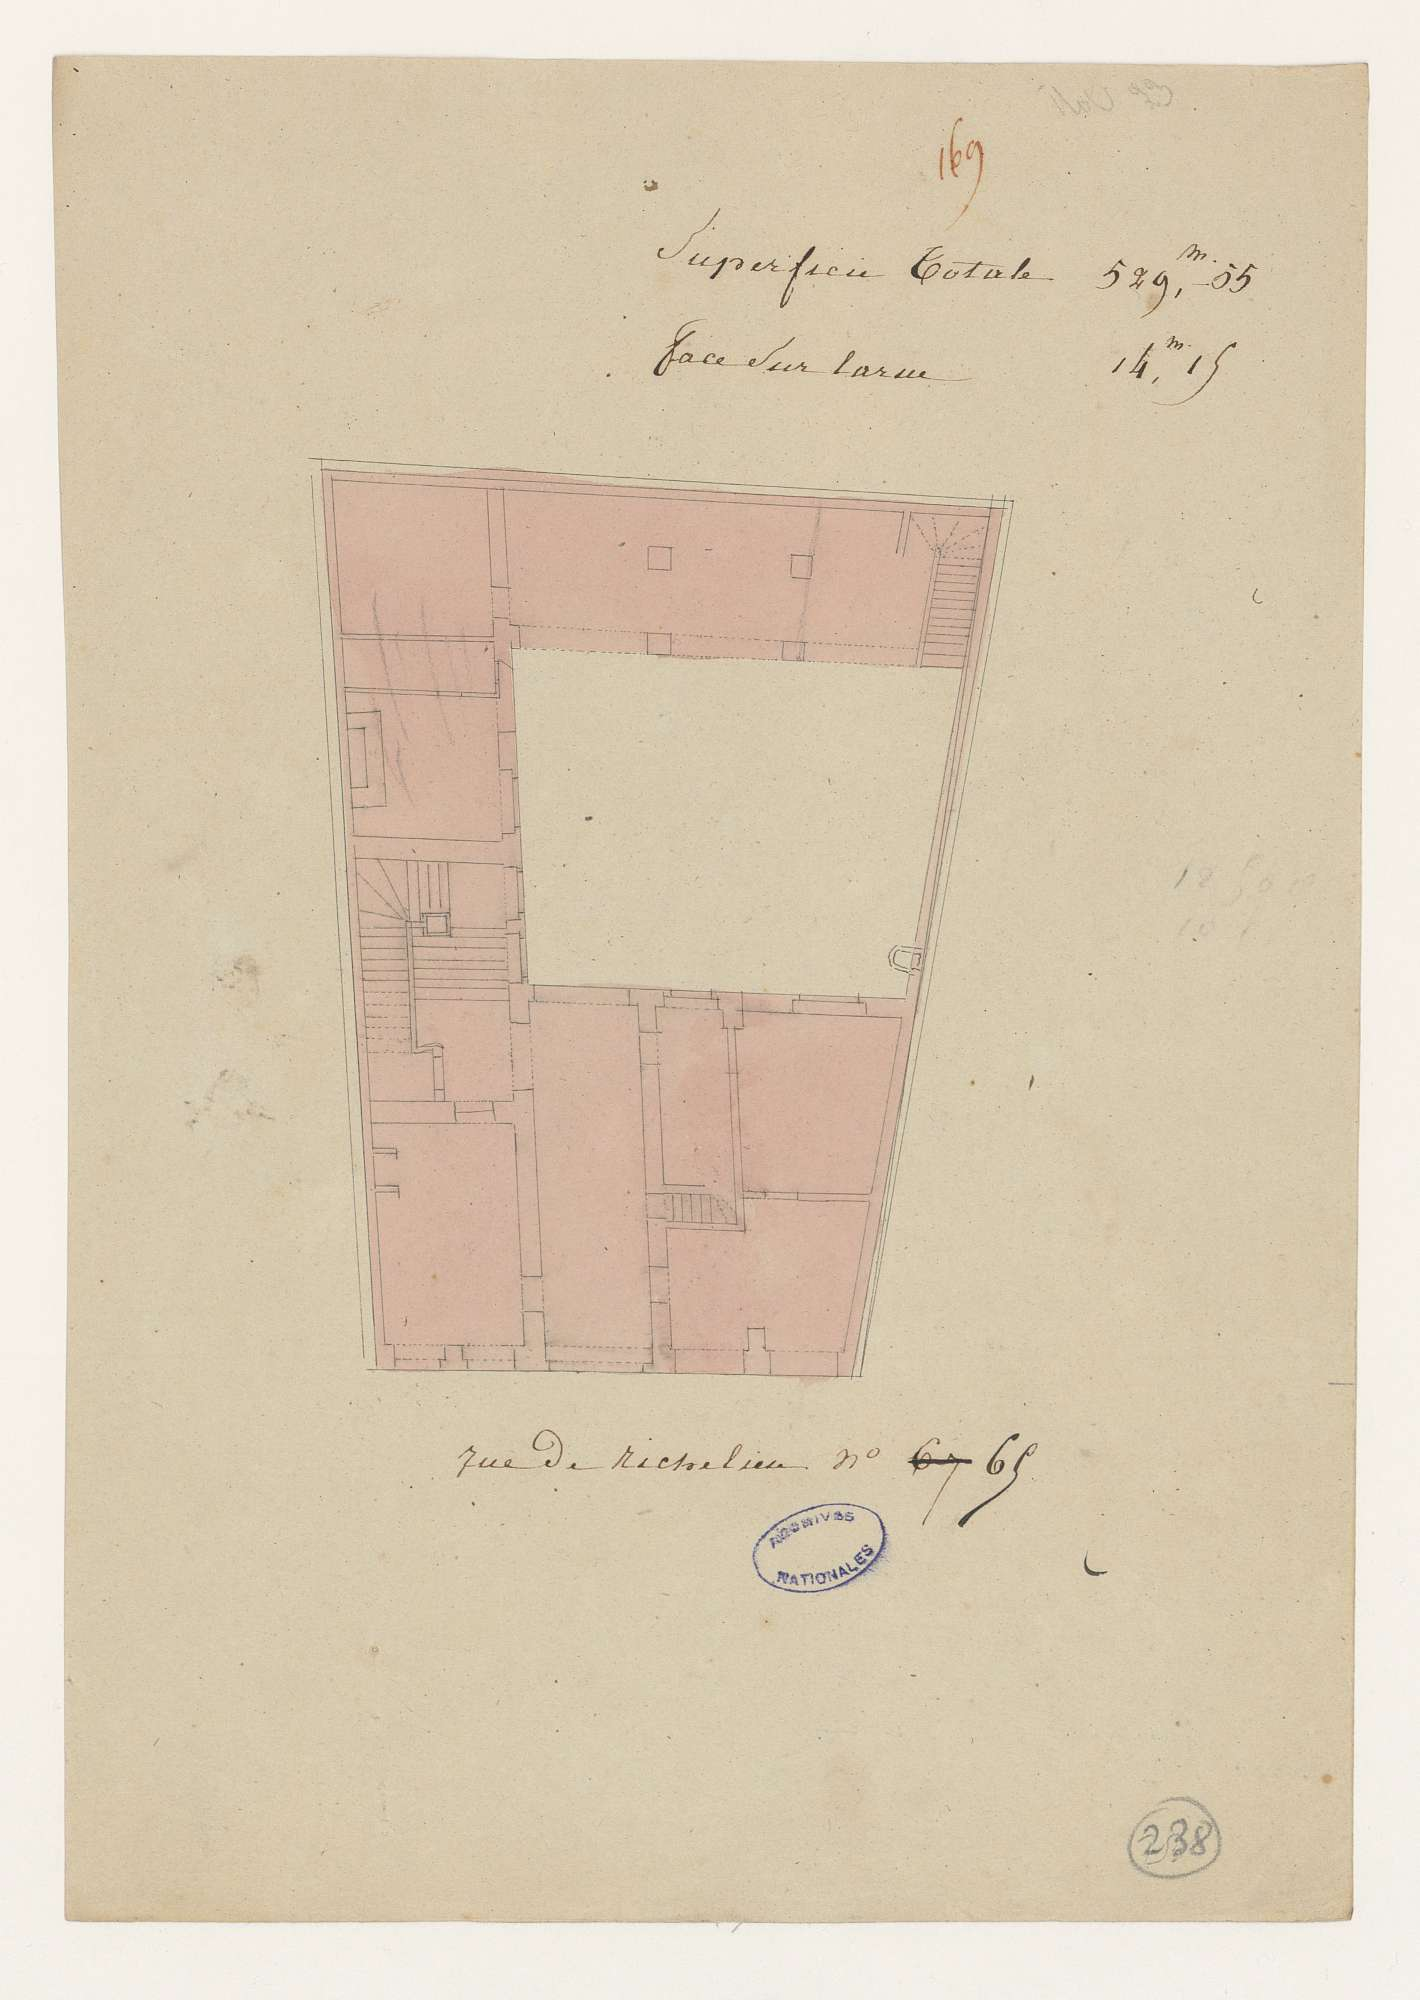
\includegraphics[width=0.5\linewidth]{images/AN_65_Richelieu.jpg}
    \caption{Plans cadastraux dit à la feuille de Paris 1809-1854, 65 rue de Richelieu, AN, \href{https://www.siv.archives-nationales.culture.gouv.fr/siv/media/FRAN_IR_058572/d_2851/FRAN_0198_3023_L}{CP/F/31/9 n°238}.}
    \label{fig:plan_carto_RR65}
\end{figure}

\begin{figure}[!]
    \centering
    \includegraphics[width=0.5\linewidth]{images/ParisMusees_Billaud.jpg}
    \caption{Plan de la Galerie et de la Rotonde Colbert, Billaud, Musée Carnavalet.}
    %\href{{https://www.parismuseescollections.paris.fr/fr/musee-carnavalet/oeuvres/plan-des-galeries-et-rotonde-colbert-conduisant-de-la-rue-vivienne-a-la-0#infos-principales}{num inv}.}
    \label{fig:plan_carto_galeries}
\end{figure}


\begin{table}[!]
\centering
\label{tab:total_carto}
    \begin{tabular}{|l|c|}
    \toprule
    \textbf{Source cartographique} & \textbf{Nombre} \\ 
    \midrule
    Contemporain & 26 \\
    Billaud & 22 \\
    Feuille & 97 \\ 
    Vasserot & 116 \\
    Parcellaire 1900 & 234 \\
    \midrule
    \textbf{Total} & \textbf{495} \\
    \bottomrule
\end{tabular} 
\caption{Calcul du nombre de documents par source cartographique.}
\end{table}

Des fonds de cartes\footcite{ESRIDefinition2024} de Paris de différentes époques viennent compléter le corpus : le plan Verniquet de 1791\footnote{Une version numérisée du plan Verniquet est disponible sur Gallica, le site \href{https://gallica.bnf.fr/view3if/ga/ark:/12148/btv1b55013275x}{ici}.}, le plan Dubrueil de 1856\footnote{Une version numérisée du plan Dubreuil est consultable sur Gallica, le lien \href{https://gallica.bnf.fr/view3if/ga/ark:/12148/btv1b53085562p}{ici}.}, et un plan municipal de 1910-1920 en cours de sélection. Ils sont tous numérisés et disponibles soit à la \acrshort{bnf} soit dans les bibliothèques spécialisées de Paris pour le plan Andriveau-Goujon de 1867.

Ces documents sont les sources primaires largement référencées et numérisées. Nous verrons par la suite quelle est la distinction que le traitement informatique effectue sur les sources cartographiques entre les plans et les fonds de carte, en raison des référentiels géohistoriques.
 
\subsubsection{Le corpus iconographique}

Le corpus iconographique s'est constitué au cours de la seconde phase du projet. L'équipe de chercheurs a effectué un repérage systématique des corpus iconographiques numérisés et conservés dans diverses institutions parisiennes et internationales. Ces documents, très variés, proviennent principalement de la \acrshort{bnf}, de l' \acrshort{inha}, de Paris Musées (dont le Petit Palais, le Musée Carnavalet, le Musée de la Vie Romantique, le Palais Galliera, la maison de Balzac, la maison de Victor Hugo, le Musée Bourdelle et le musée de la Libération Leclerc Moulin), ainsi que des Archives nationales, des Archives de la Ville de Paris, des bibliothèques spécialisées de Paris, et du British Museum. Les représentations graphiques, telles que les photographies, cartes postales, estampes, gravures (voir la figure \ref{fig:palais_royal1789}), dessins, croquis d'architectes et même peintures (voir la figure \ref{fig:clair_lune}), offrent un aperçu visuel de différentes époques, capturant l'architecture, l'aménagement des rues (voir la photographie \ref{fig:urinoir}), les événements, les passants, et parfois des scènes de la vie quotidienne. En plus de cela, des documents comme des coupures de presse, des affiches publicitaires, ainsi que des éléments plus inattendus tels que des jetons de commerce, des menus de restaurant, et des cartes de visite ont été sélectionnés. Au total, plus d'une centaine de typologies différentes forment un corpus iconographique hétérogène, rassemblant un total de plus de 5000 documents (voir le tableau \ref{tab:iconographie_institution}).

\begin{figure}[ht!]
    \centering
    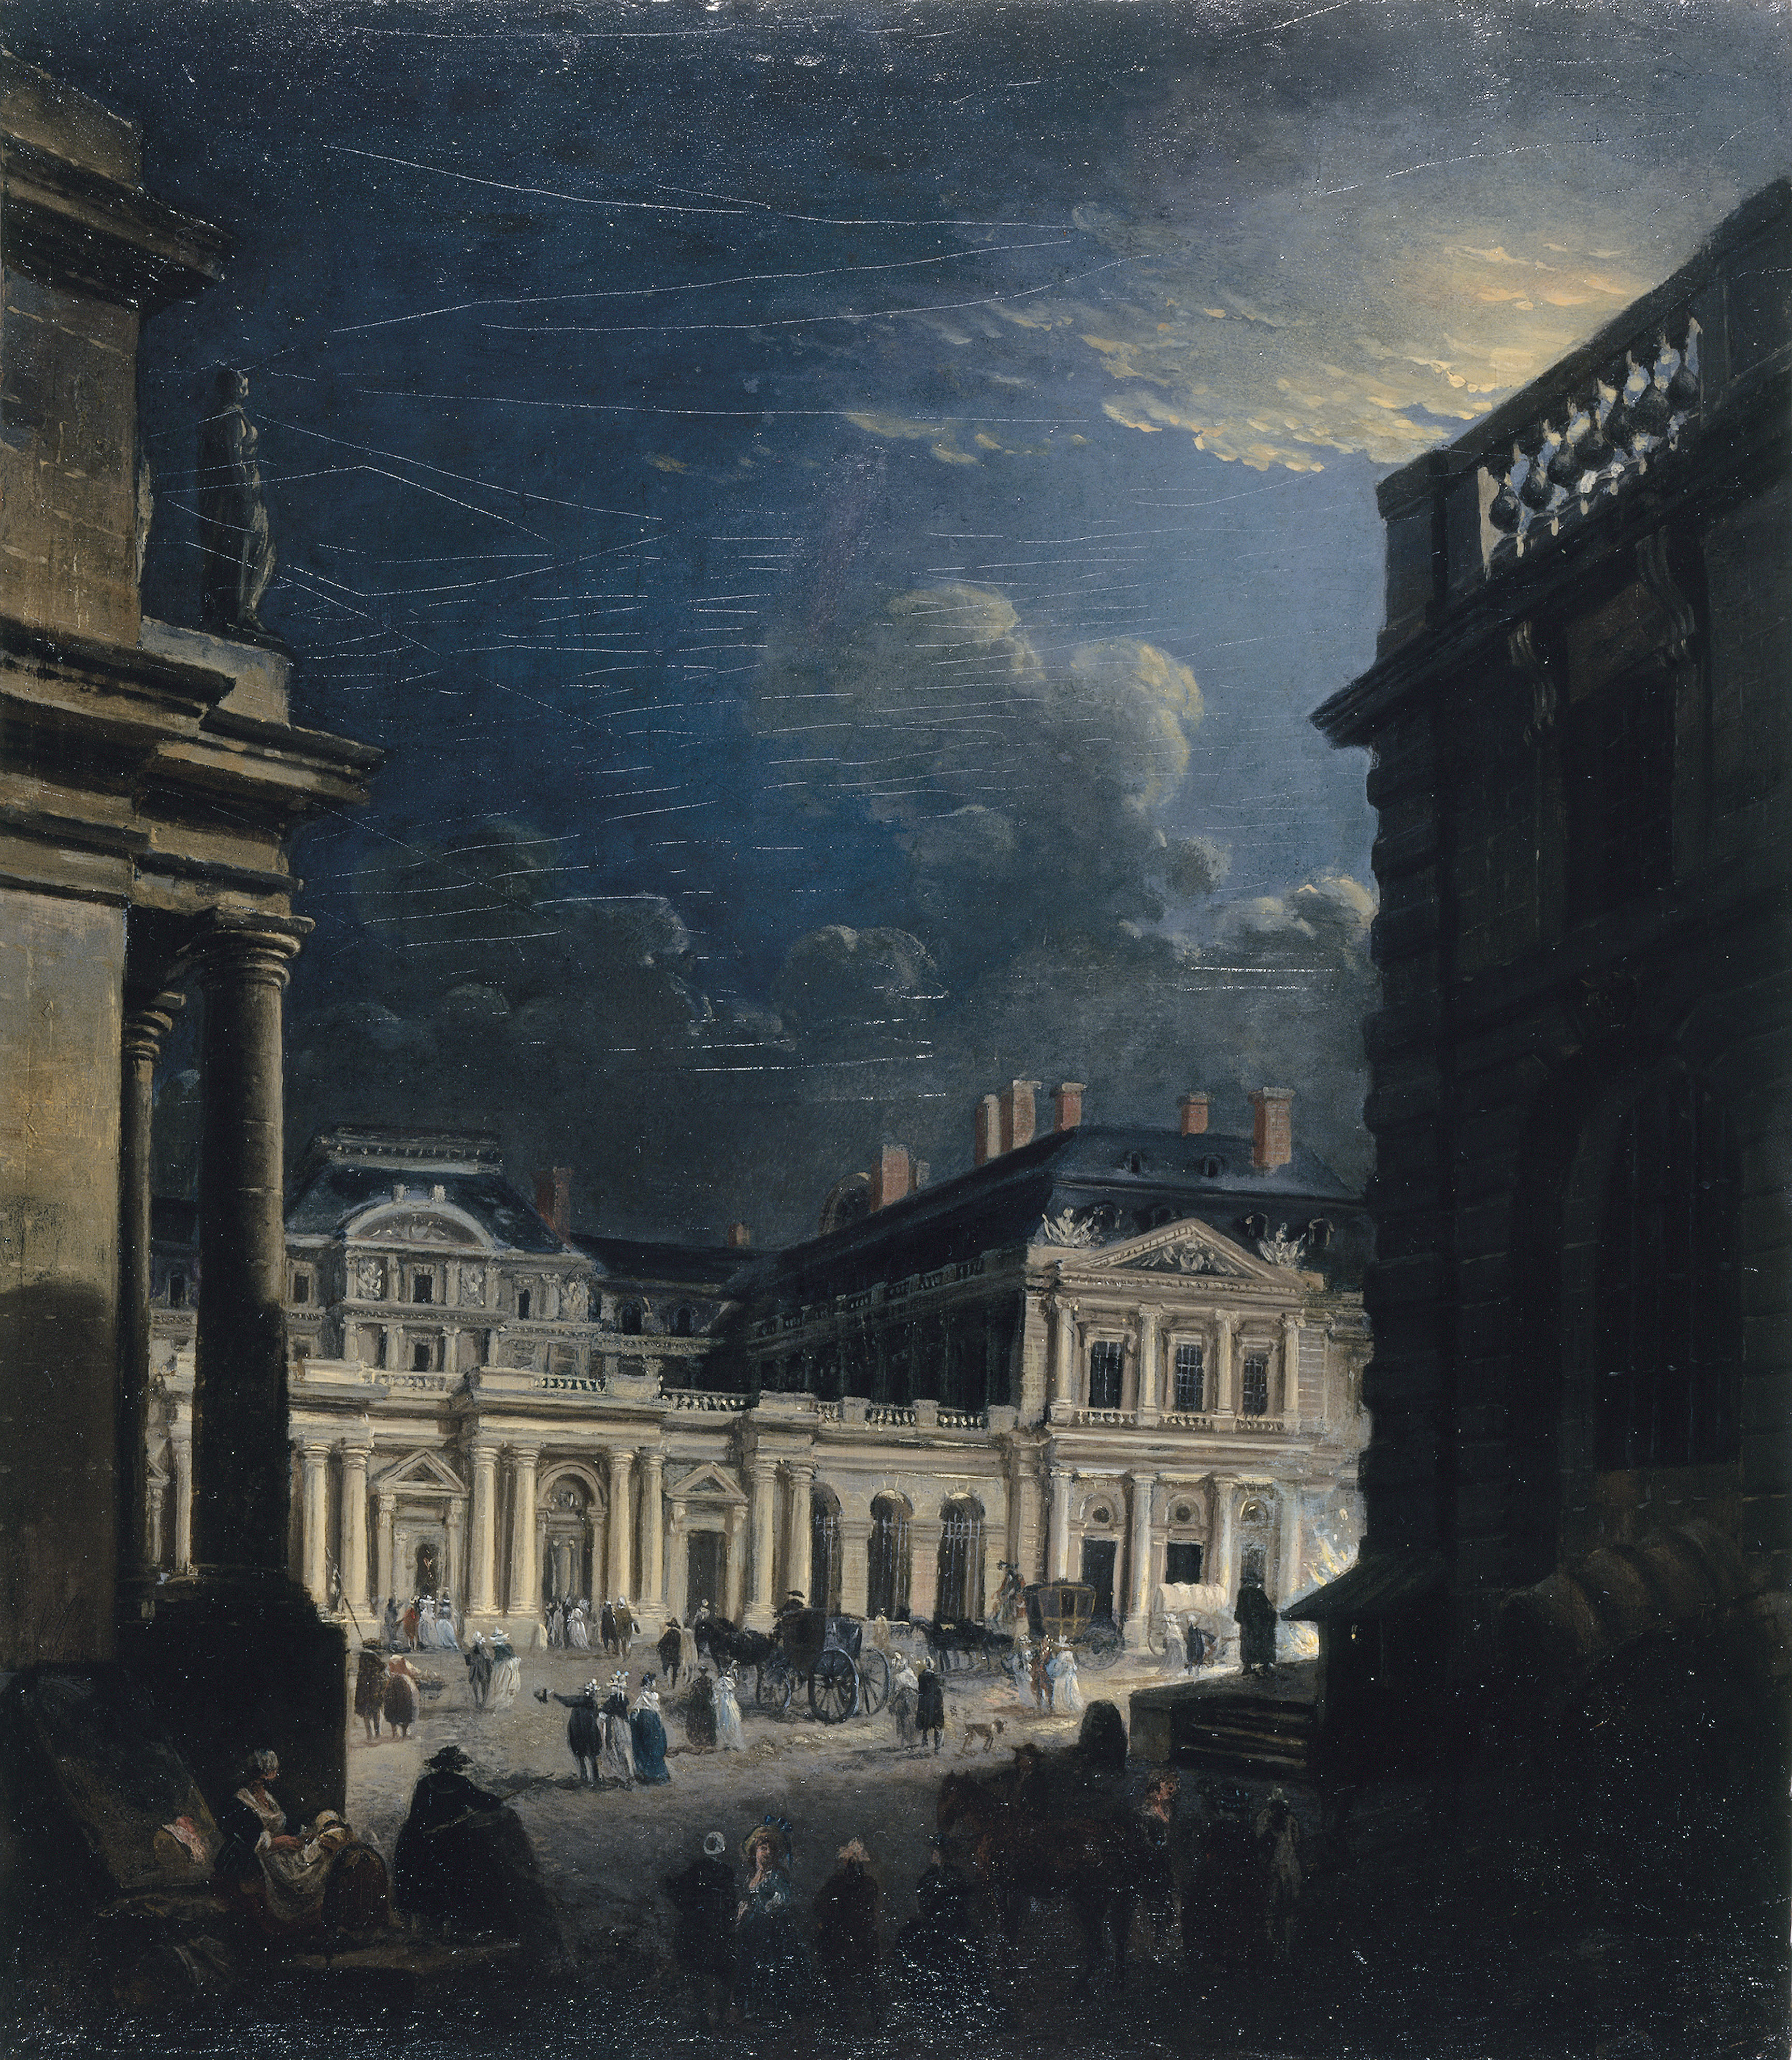
\includegraphics[width=0.5\linewidth]{images/palais_royal_clairdelune.jpg}
    \caption{Pierre-Antoine Demachy (1723 - 1807), \textit{La Place du Palais Royal, au clair de lune}, vers 1765, Huile sur toile, 39,5 x 34 cm, Musée Carnavalet, P93.}
    \label{fig:clair_lune}

%https://www.parismuseescollections.paris.fr/fr/musee-carnavalet/oeuvres/la-place-du-palais-royal-au-clair-de-lune#infos-secondaires-detail 
\end{figure}
\begin{figure}[ht!]
    \centering
    \includegraphics[width=0.7\linewidth]{images/vue_palais_royal1789.jpg}
    \caption{Première vue du jardin du Palais Royal, prise de la Rotonde, Paris, Aubert, 1789, Musée Carnavalet,  }
    \label{fig:palais_royal1789}
\end{figure}

\begin{figure}[ht!]
    \centering
    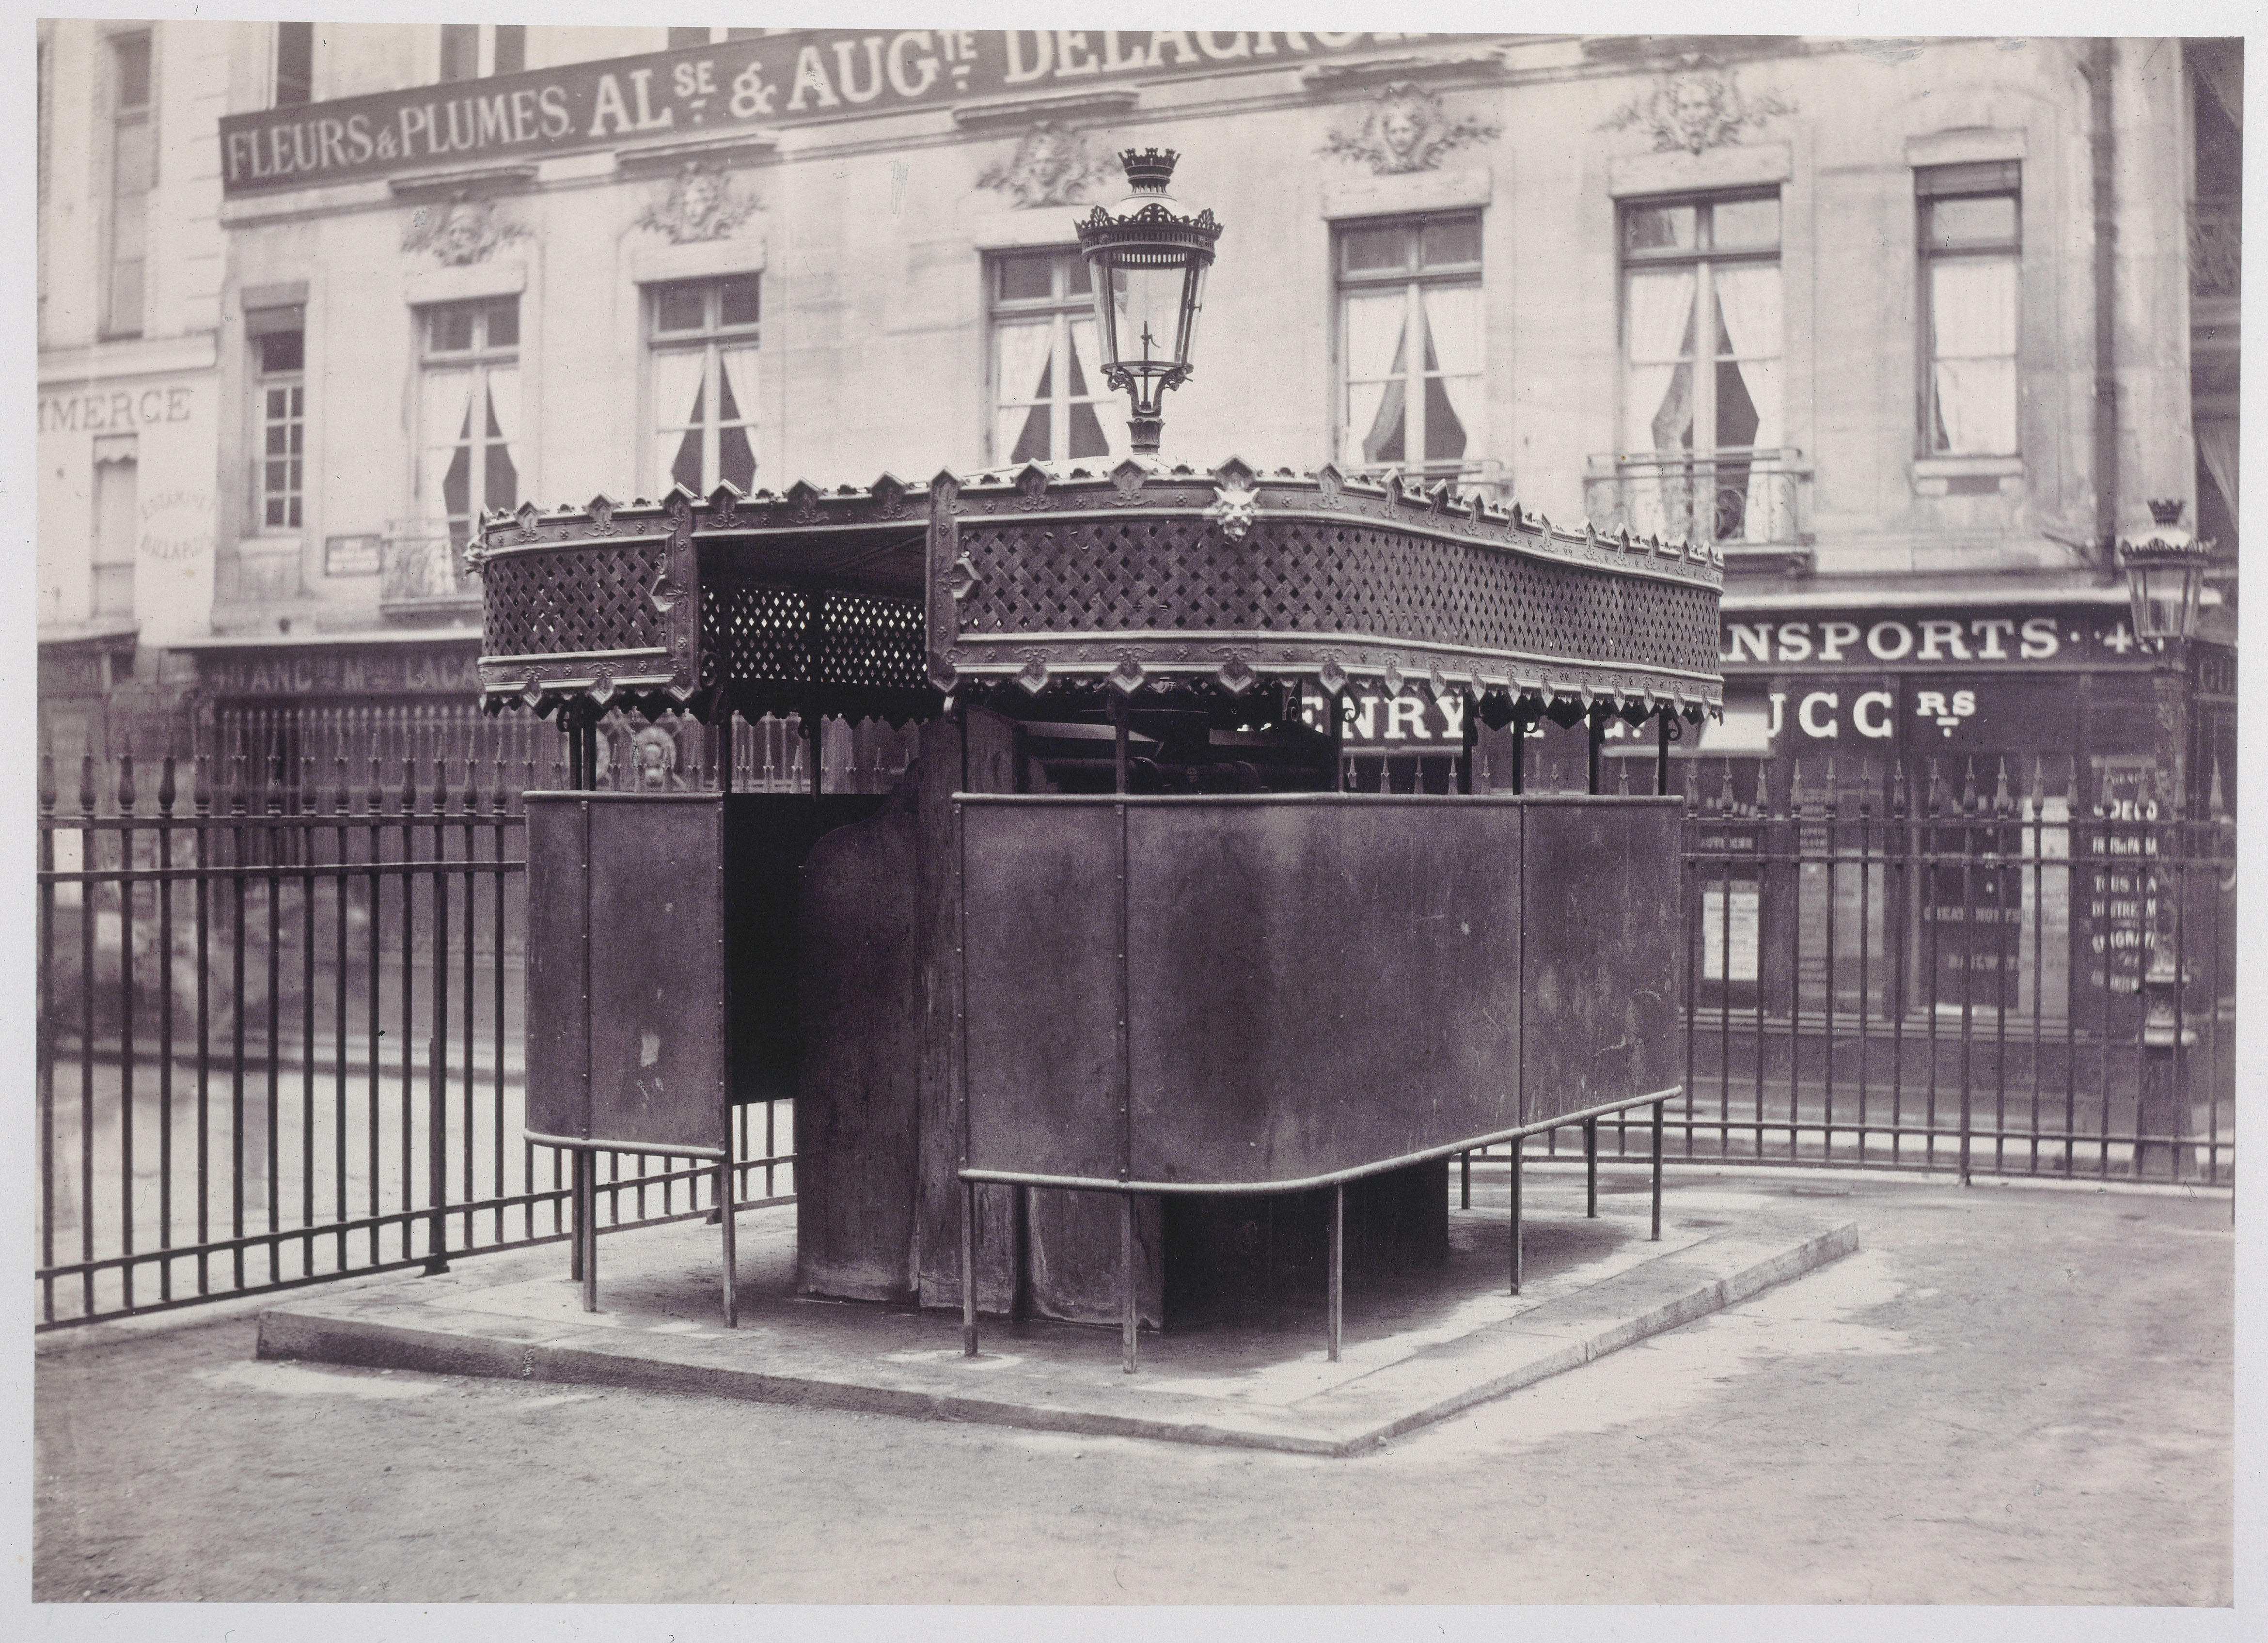
\includegraphics[width=0.7\linewidth]{images/urinoir_marville.jpg}
    \caption{Urinoir enveloppé à six stalles, jardin de la Bourse, place de la Bourse, Paris, Marville, photographie, seconde moitié du XIX\ieme~ siècle, Musée Carnavalet, PH4147.}
    \label{fig:urinoir}
\end{figure}

% \begin{figure}[ht!]
%     \centering
%     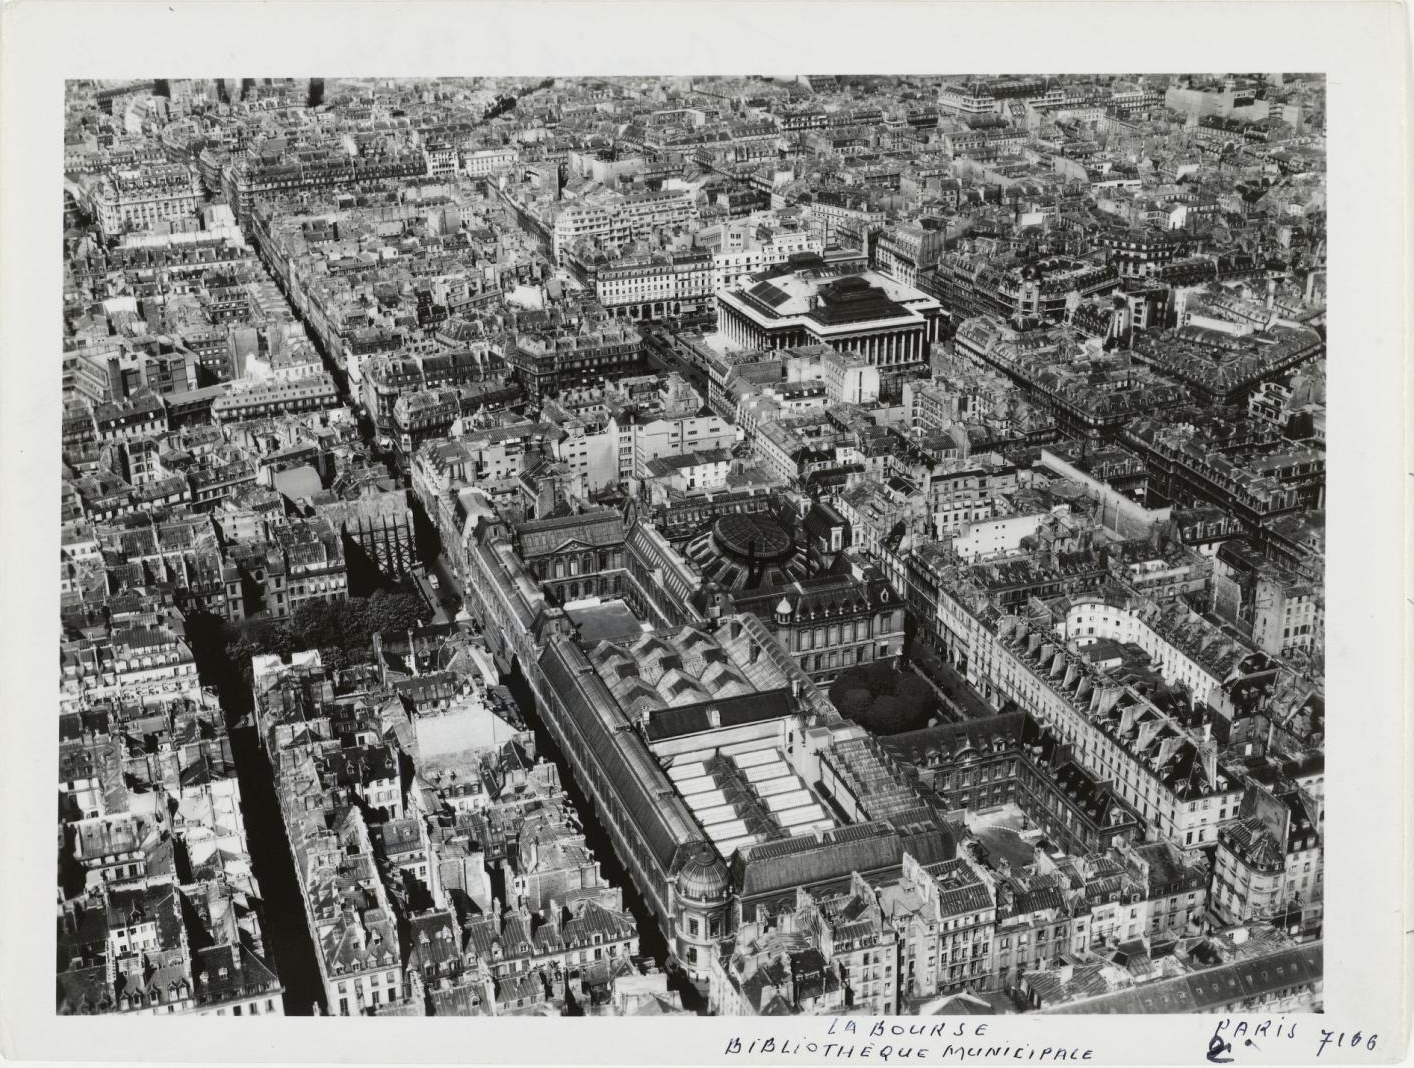
\includegraphics[width=1\linewidth]{images/vue_aerienne.png}
%     \caption{\href{https://www.parismuseescollections.paris.fr/fr/musee-carnavalet/oeuvres/vue-aerienne-de-paris-la-bourse-des-valeurs-palais-brongniart-et-la}{Vue aérienne de Paris} : la Bourse, le palais Brongniart et la Bibliothèque nationale, rue de Richelieu, Paris, Roger, photographie, 1952, Musée Carnavalet, PH344-7166.}
%     \label{fig:vue_aerienne}
% \end{figure}

\begin{table}[ht!]
\centering
\begin{tabular}{|l|c|c|}
\toprule
\textbf{Lieux de conservation} & \textbf{Nombre} & \textbf{Nombre} \\
\midrule
Musée Carnavalet & & 1333 \\
Bibliothèque nationale de France & 1312 & \\
Bibliothèques spécialisées de la Ville de Paris & 928 & \\
Bibliothèque historique de la Ville de Paris & 827 & \\
British Museum & 295 & \\
Institut national d'histoire de l'art & 162 & \\
Bibliothèque Forney & 73 & \\
Archives de Paris & 46 & \\
Palais Galliera & & 37 \\
Maison de Balzac & & 31 \\
Musée Albert Kahn & 30 & \\
Maison Victor Hugo & & 27 \\
Bibliothèque de l'Hôtel de Ville & 16 & \\
Bibliothèque Marguerite Durand & 5 & \\
Petit Palais. Musée des Beaux-Arts de la Ville de Paris & & 4 \\
Bibliothèque municipale et patrimoniale Villon & 4 & \\
Bibliothèque des littératures policières & 4 & \\
Musée de la Libération Leclerc Moulin & & 4 \\
Médiathèque Marguerite Duras & 2 & \\
Bibliothèque du tourisme et des voyages - Germaine Tillion & 2 & \\
Médiathèque musicale de Paris & 1 & \\
Musée de la Vie Romantique & & 1 \\
Musée Bourdelle & & 1 \\
\midrule
SOUS-TOTAL Paris Musées & & 1438 \\
\textbf{TOTAL} &  \textbf{5145} & \\
\bottomrule
\end{tabular}
\caption{Répartition du corpus iconographique par lieu de conservation}
\label{tab:iconographie_institution}
\end{table}

\newpage

Force est de constater que la numérisation partielle des collections par certaines institutions limite l'exhaustivité matérielle et historique d'un projet de recherche. Bien que la numérisation ait permis un accès inédit à une vaste quantité de documents, elle ne couvre qu'une portion des archives disponibles, laissant de côté des ressources certainement essentielles pour une constitution complète de l'histoire du quartier. Toutefois, cela est suffisant pour apporter un échantillon représentatif du quartier. Cette situation souligne non seulement les contraintes documentaires avec lesquelles le projet Richelieu s'est développé, mais elle constitue aussi un appel à élargir les chantiers de numérisation au sein des institutions patrimoniales, notamment pour le développement des bibliothèques numériques.\footnote{A titre d'exemple, l'ENC a pour ambition de numériser l'ensemble de ses archives et documents afin de créer une bibliothèque numérique. Le chantier, en fonction des financements, devrait être lancé à l'automne 2024.} 

\subsection{Les corpus secondaires}
\subsubsection{Le corpus textuel}
Ce corpus est principalement constitué de bottins, almanachs du commerce et anciens répertoires d'adresses. Ce type de publications proposant des listes d'adresses de commerçants, fabricants, industriels, etc. centrées sur un espace urbain donné est un genre en pleine expansion au XIX\ieme~  siècle. Ces ouvrages collectionnent et intègrent une masse d'informations qui ne cesse d'augmenter et de se diversifier tout au long de la période. Ils constituent aussi et surtout de véritables objets spatiaux et sociaux qui témoignent de l'évolution de la société. Les ensembles de références spatiales indirectes qu'ils contiennent (les adresses et localisations en tout genre) accompagnent et décrivent le développement des villes – notamment celle de Paris – , et l'augmentation de leur population. Ils exposent de manière fine les concentrations et les évolutions du commerce, de l'artisanat et de l'industrie, tout en témoignant de la société dans son ensemble. L'exploitation de ces informations de localisation en grand nombre constitue une source privilégiée pour étudier sur le long terme l'évolution des dynamiques sociales en contexte urbain, qui plus est à différentes échelles et niveaux d'observation et d'analyse. \footnote{L'étude est les méthodologies numériques d'analyse ont fait l'objet d'une journée d'études à la \acrshort{bnf} : \footcite{BNFJournee2022}}

Pour le projet Richelieu, le parti pris était de définir les métiers exercés dans le quartier. Les sources sont principalement issues de la \acrshort{bnf}. Au total, 56 annuaires datant de 1839 à 1922 ont été océrisé (\acrshort{ocr}) pour un volume considérable de données : 4 millions d'adresses dans tout Paris sont extraites des 27 000 pages. Nous verrons par la suite le devenir de ce corpus au sein du projet Richelieu dont le traitement et l'alignement des données en dépend. 

\subsubsection{Le modèle \acrshort{3d} historique}  
En complément des autres corpus, le projet a travaillé sur la constitution d'un modèle \acrshort{3d} historique. S'inspirant de projets analogues\footcite{GOUET-BRUNETIndexation2023a}, un relevé lasergrammétrique a été entrepris avec Plemo \acrshort{3d}. A partir de-là, et en inspiration au procédé photogrammétrique, le travail a consisté à replacer les vues représentatives d'un objet physique afin de montrer l'évolution architecturale à travers le temps. Ce travail s'est concentré sur la place de la Bourse au XIX\ieme~ siècle qui est aménagée sous le Premier Empire pour accueillir le Palais Brongniart à l'emplacement de l'ancien couvent des Filles-Saint-Thomas. Elle marque une étape décisive dans l'urbanisation du quartier : elle conditionne le prolongement de la rue Vivienne et devient un des épicentres économiques de la vie parisienne. Le travail s'appuie sur la collecte de 700 documents iconographiques (gravures, dessins, photos, plans) documentant l'évolution de la place entre 1810 et 1950. Un \acrlong{sig} (SIG) est utilisé pour spatialiser ces données dont les dimensions ne sont pas que la latitude et la longitude, sinon l'altitude et l'orientation de la prise de vue également. L'intégration de ce travail, à comprendre comme un modèle \acrshort{3d} enrichi de données historiques, au projet final est en cours d'interrogation. 

\subsubsection{Pour aller plus loin}
Reconstituer un quartier dans toutes ses dimensions est une entreprise ambitieuse. Pour ce faire, diverses sources peuvent enrichir l'analyse du quartier.

Les archives textuelles et administratives, telles que les permis de construire, les plans d'urbanisme, les recensements, les registres de propriété et les rapports municipaux constituent des sources d'informations pour l'étude du quartier. Les documents commerciaux et publicitaires, comme les annuaires et les guides, renseignent sur les activités économiques des commerces et entreprises, ainsi que sur l'évolution des habitudes de consommation. De plus, les registres de l'état civil et paroissiaux fournissent des données sur l'histoire démographique et permettent d'examiner les dynamiques familiales, sociales et sociologiques. Les articles de presse et les journaux constituent également une source précieuse : ils relatent des événements historiques et faits divers, présentent des annonces, des critiques et des témoignages sur l'histoire du quartier. La littérature, quant à elle, offre des perspectives subjectives mais souvent riches sur la vie quotidienne à travers des descriptions littéraires, des récits de voyageurs et des mémoires. Enfin, bien que sortant du cadre traditionnel de l'analyse documentaire, les éléments tels que le son, l'image animée, le film, ainsi que les sensations comme l'odeur et le goût de la ville moderne, peuvent également offrir des perceptions originales du quartier. Quelques unes de ces diverses pistes de réflexion ont animé les séminaires du projet et fournissent ainsi une multitude de perspectives sur le quartier à travers le temps.

\subsubsection{Conclusion}
En conclusion, l'exploration documentaire entreprise dans le cadre du projet Richelieu témoigne d'une ambition d'exhaustivité pour reconstituer l'histoire du quartier sur une période de deux siècles. La fouille des sources historiques, tant cartographiques qu'iconographiques, a permis de rassembler un ensemble de documents de natures différentes et essentiels pour visualiser l'évolution du quartier Richelieu. Cependant, la sélection des sources a été orientée par la contrainte de numérisation, limitant ainsi l'accès aux archives disponibles. Cette réalité met en lumière les défis liés à la recherche historique dans un contexte de numérisation partielle des collections. Finalement, la diversité des sources mobilisées, qu'elles soient cartographiques, iconographiques ou textuelles, enrichit considérablement la compréhension de l'histoire complexe et multifacette du quartier, offrant ainsi une approche multidimensionnelle et profondément ancrée dans le temps.


%%%%%%%%%%%%%%%%%%%%%%%%%%%%%%%%%%%%%
% SECTION %%%%%%%%%%%%%%%%%%%%%%%%%%%
\section{Définition des objectifs techniques}
Quels sont les objectifs du projet ? Que signifie pour les acteurs \enquote{investiger sur l'histoire de son quartier}? Comment cette investigation se concrétise-t-elle ?  Quelle forme prend-elle ? Quel est le développement informatique attendu ? Le but de cette sous-partie ici est de confronter les attentes initiales, telles que décrites dans les documents officiels, aux réalisations effectivement privilégiées afin de comprendre le moment dans lequel s'intègre le stage. Ce passage est réalisé à partir d'une étude comparative des appels à financements de projets de recherche auprès de la Fondation des sciences du Patrimoine qui distribuent de nombreux fonds\footnote{Pour plus d'informations, consulter la page : https://www.sciences-patrimoine.org/recherche/appel-a-projets/ }. 

Depuis le lancement du projet en 2018 jusqu'à sa finalisation prévue en 2024, l'objectif est demeuré constant : explorer les diverses dimensions de l'histoire du quartier (urbanistique, architecturale, économique, administrative, sociologique, culturelle) et concevoir un modèle innovant d'exploration des données patrimoniales à travers quatre axes principaux : le temps, l'espace, le réseau social, et l'iconographie. Comment se représenter cette innovation ? Les ingénieurs ont-ils accompagné les chercheurs pour cette définition ? Bien que cet objectif soit ambitieux, il reste clair. Un \enquote{système d'information innovant}\footcite{PROJETFondation2021} est souvent évoqué pour atteindre ce but, mais les détails techniques manquent dans l'appel à projet de 2021. Des concepts sont énumérés tels qu'un modèle conceptuel d'informations multidimensionnelles, l'ontologie \acrshort{cidoc}, le modèle de données d'annotation Web, le VIR, les représentations \acrshort{3d}, les informations cartographiques \acrshort{2d}, ainsi que l'intégration avec le Web de données et des autorités externes (Wikidata, Getty) sont mentionnés. De plus, l'exploration des données au format \acrshort{rdf} du Web sémantique à travers une plateforme utilisant \acrshort{sparql}, et l'implémentation d'Aïoli pour la plateforme \acrshort{3d}, sont également citées. 
Lors de l'appel à projet de 2023, le périmètre du projet a été redéfini et les ambitions sémantiques ont été remises en cause. Les objectifs sont le développement d'un outil d'exploration des données via une application Web servant d'\enquote{exposition finale des corpus du projet Richelieu}\footcite{PROJETFondation2023}. Une carte est d'ores et déjà attendue. Un catalogue iconographique l'est également. Le développement de cette application nécessite une chaîne robuste pour le traitement des données, qui sera présentée dans le chapitre suivant.

\subsubsection{Conclusion du chapitre}
Ce premier chapitre introductif a permis de poser le cadre du projet de recherche en présentant son contexte historique, son objet d'étude, ses acteurs, ses objectifs, ainsi que les corpus de recherche mobilisés. En inscrivant le projet Richelieu dans une démarche interdisciplinaire, il s'agit non seulement de comprendre l'émergence de l'archétype de la capitale moderne, et surtout de proposer une nouvelle clé de lecture du quartier Richelieu, en s'appuyant sur des collaborations nationales et internationales enrichissant l'écosystème de l' \acrshort{inha}. L'ambition du projet réside dans sa volonté de reconstituer l'histoire du quartier Richelieu sur une période de deux siècles, en utilisant une exploration documentaire et archivistique exhaustive. En dépit de ces contraintes, la diversité des sources mobilisées enrichit considérablement la compréhension du quartier Richelieu, offrant une perspective multidimensionnelle sur son histoire complexe. Le projet Richelieu, à travers le développement d'un outil d'exploration des données, se positionne comme une initiative pionnière pour approfondir notre connaissance de l'urbanisation parisienne et des dynamiques qui ont façonné ce quartier emblématique.